\chapter{Decision Trees}

Let's start with training set:
\dfn{
Training set
}{
    is defined training set a \textit{set of examples}, where:
    \begin{math}
        \langle x^{(i)}, y^{(i)} \rangle
    \end{math}
    where:
    \begin{itemize}
        \item \textit{i} is the instance of the example 
        \item $x^{(i)}\in X$ is the set of \textit{input} 
        \item $y^{(i)}\in Y$ is the set of \textit{output}
    \end{itemize}
}

the problem of machine learning is to find a function $h:X\to Y$ that approximates the real function $f:X\to Y$. We have two types of problems:
\begin{itemize}
    \item \textbf{Classification}: $Y$ is a discrete set of values (e.g. $\{0,1\}$)
    \item \textbf{Regression}: $Y$ is a continuous set of values (e.g. $\mathbb{R}$)
\end{itemize}
\section{Hypothesis space}

In machine learning the \textit{hypothesis space} $H$ is defined as the set of all possible functions that can be used to approximate the real function $f:X\to Y$. Formally:
\dfn{
Hypothesis space
}{
    A hypothesis space $H$ is defined as the set:
    \begin{math}
        H = \{h | h:X\to Y\}
    \end{math}
    where:
    \begin{itemize}
        \item $h$ is a function (hypothesis) that maps input $X$ to output $Y$
        \item $X$ the input space (features, domain of data).
        \item $Y$ the output space (labels, range of data).
        \item $|H|$ is the size of the hypothesis space (number of possible hypotheses)
    \end{itemize}
}
this let us to define the model:
\dfn{
Model
}{
    A model is a way to compute a function $h\in H$ from the training set.
}

\ex{
    Decision tree
}{
    A good day to play tennis? Our function $F$ is:
    \[
        \mathbb{F}:Outlook \times Humidity \times Wind \times Temp \to Play Tennis?
    \] 
    \begin{center}
        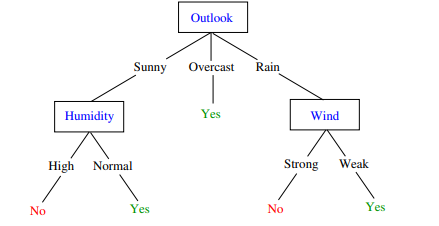
\includegraphics[width=0.6\textwidth]{dtree.png}
    \end{center}
    where:
    \begin{itemize}
        \item $Outlook\in\{Sunny, Overcast, Rain\}$
        \item $Humidity\in\{High, Normal\}$
        \item $Wind\in\{Weak, Strong\}$
        \item $PlayTennis?\in\{Yes, No\}$
    \end{itemize}

    Every node tests an attribute. Each branch corresponds to one of the possible values for that attribute. Each leaf node assigns a classification (Yes or No), in other words predicts the answer $Y$.

    The prblem configurationg is the following:
    \begin{itemize}
        \item $X$ is the set of all possible $x\in X$ that corresponds to a vector of attributes $(Outlook, Humidity, Wind, Temp)$ 
        \item Target function $f:X\to Y$ is the function that maps the attributes to the target variable $PlayTennis?$ (booleans)
        \item Hypothesis space $H=\{h | h:X\to Y\}$ is the set of all possible decision trees that can be constructed using the attributes in $X$ to predict the target variable $Y$
    \end{itemize}

    \begin{center}
        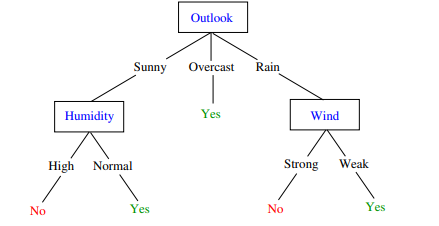
\includegraphics[width=0.6\textwidth]{dtree.png}
    \end{center}
}

\subsection{Top-down inductive construction}
Let $X = X_1 \times X_2 \dots \times X_n $ where $X_i = \{\text{Truee},\text{False}\}$


Can we represent, for instance, $ Y = X_2 \land X_5$? or $Y=X_2 \land X_5 \lor (\lnot X_3) \land X_4 \land X_1 ? $

and:

\begin{itemize}
    \item do we have a decision tree for each h in the space hypothesis?
    \item if the tree exists, is it unique?
    \item if it is not unique, do we have a preference?
\end{itemize}

\thm{
    Basta - Bonzo
}{
    Main loop:
    \begin{itemize}
        \item \textbf{Pick the "best" attribute $X_i$}: At the current node, choose which featue/attribute will bwst split the training data.
        
        Best means: the attribute that gives the most information gain
        \item \textbf{Create a child node for each possible value of $X_i$}: for instance if attribute is "weather" with values "sunny", "rainy", "overcast", create three child nodes.
        \item \textbf{check if all examples in the chils node are pure}: if all examples belong to the same class (e.g., all "yes" or all "no"), make that node a leaf node with that class label. If not repeat the process recursively for each child node.
    \end{itemize}
}

\subsection{Entropy}

\dfn{
    Entropy
}{
    The entropy $H(S)$ of a set of examples $S$ is defined as:
    \[
        H(S) = -\sum_{i=1}^{n} P(X=i)\log_2 P(X=i)
    \]
    where:
    \begin{itemize}
        \item $P(X=i)$ is the proportion of examples in $S$ that belong to class $i$
        \item $n$ is the number of classes (the number of possibile values of $X$)
    \end{itemize}
}

In other words, Entropy meausers the \textit{degree of uncertainty} of the information. It is maximal when $X$ is uniformly distributed (all classes have the same probability) and minimal (zero) when all examples belong to the same class (pure set)
\begin{center}
    \IfFileExists{imgs/entropy.png}{%
        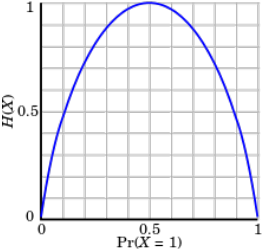
\includegraphics[width=0.6\textwidth]{imgs/entropy.png}%
    }{%
        \fbox{\parbox{0.6\textwidth}{\centering Missing image: imgs/entropy.png}}%
    }
\end{center}

\subsubsection{Information Theory (Shannon 1948)}
The entropy is the average amount of information produced by a stochastic source of data. The \textit{information} is associated to the \textit{probability} of each datum (the surprise element):
\begin{itemize}
    \item An event with probability 1 (certain event) provides no information (no surprise): \(I(1)=0\).
    \item An event with probability 0 (impossible event) provides infinite information (really surprising): \(I(0)=\infty\).
    \item Given two independent events \(A\) and \(B\), the information provided by both events is the sum of the information provided by each event:
    \[
        I(A \cap B) = I(A) + I(B)
    \]
\end{itemize}
So is natoral defining 
\[
    I(p) = -\log_2(p)
\]
\subsubsection{Code Theory (Shannon-Fano 1949, Huffman 1952)}
The entropy is also related to the avarage number of bits required to transmit outcomes produces by a stochastic source process $x$.

Let suppose to have $n$ events with same probability \(p_i = \frac{1}{n}\). Home many bits do we need to encode these events? The answer is \(\log_2(n)\) bits. For instance, if we have 4 events, we need 2 bits to encode them:.

In this case:
\[
    H(X) = -\sum_{i=1}^{n} P(X=i)\log_2 P(X=i) = - \sum_{i=1}^{n} \frac{1}{n} \log_2 \frac{1}{n} = \log_2(n)
\]

\subsection{Information Gain}

In a decision tree, the goal is to maximize the information gain during the execution of the algorithm. 
In other words, the final split should result in the minimum possible impurity. 
Here are the main formulas:

\thm{Entropy of $X$}{
    \[
        H(X) = -\sum_{i=1}^{n} P(X=i)\log_2 P(X=i)
    \]
}

\thm{Conditional Entropy of $X$ given a specific $Y=v$}{
    \label{thm:cexyv}
    \[
        H(X \mid Y=v) = -\sum_{i=1}^{n} P(X=i \mid Y=v)\log_2 P(X=i \mid Y=v)
    \]
}

This measures the entropy of $X$ restricted to the subgroup where $Y=v$.

\thm{Conditional Entropy of $X$ given $Y$}{
    \[
        H(X \mid Y) = \sum_{v=1}^{m} P(Y=v) \, H(X \mid Y=v)
    \]
}

This is the generalization of \ref{thm:cexyv}, used to evaluate the utility of an attribute. 
It measures the average impurity that remains in $X$ after splitting the data using all possible values of $Y$.

\thm{
    Information Gain between $X$ and $Y$
}{
    Here we are!
    \begin{math}
        I(X, Y ) = H(X) - H(X\|Y ) = H(Y ) - H(Y \|X)
    \end{math}
}

\ex{Information gain}{
    Let us measure the entropy reduction of the target variable $Y$ due to some attribute $X$, that is the information gain $I(Y , X)$ between $Y$ and $X$

    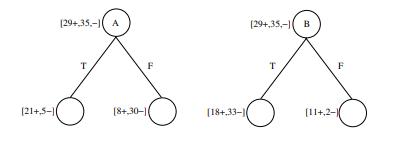
\includegraphics{ig.png}

    \[
    \begin{aligned}
    H(Y) &= -\frac{29}{64}\log_2\!\left(\tfrac{29}{64}\right) - \frac{35}{64}\log_2\!\left(\tfrac{35}{64}\right) = 0.994 \\[6pt]
    H(Y \mid A=T) &= -\frac{21}{26}\log_2\!\left(\tfrac{21}{26}\right) - \frac{5}{26}\log_2\!\left(\tfrac{5}{26}\right) = 0.706 \\[6pt]
    H(Y \mid A=F) &= -\frac{8}{38}\log_2\!\left(\tfrac{8}{38}\right) - \frac{30}{38}\log_2\!\left(\tfrac{30}{38}\right) = 0.742 \\[6pt]
    H(Y \mid A) &= 0.706 \cdot \tfrac{26}{64} \;+\; 0.742 \cdot \tfrac{38}{64} = 0.726 \\[6pt]
    I(Y, A) &= H(Y) - H(Y \mid A) = 0.994 - 0.726 = 0.288 \\[6pt]
    H(Y \mid B) &= 0.872 \\[6pt]
    I(Y, B) &= 0.122
    \end{aligned}
    \]
}

% TODO: LA PARTE DELLA CONITINUITÀ
\chapter{Overfitting}
Let us consider the error of the hypothesis $h$
\begin{itemize}
    \item on the training set, $error_{train}(h)$
    \item on the full data set $\mathcal{D}$, $error_{\mathcal{D}}(h)$ 
\end{itemize}

\dfn{Overfitting}{
    It's said taht $h$ \textit{overfits} the training set if there exixsts another
     hypotheses $h'$ such that:
     \[
        \et{h}<\et{h'}
     \]
     but
    \[
        \ed{h} > \ed{h'}
    \]
}

These models ($h$ and $h'$) represent two different situations.
The first corresponds to a model that fits the training dataset very closely, including its uncertainty and noise.
The second is simpler: it captures only the general trend of the training data and avoids fitting the noise.
As a consequence, the error with respect to the true data distribution $\mathcal{D}$ is larger for the first model than for the second.
The second one is better! Let's generalised.

But \textit{We do not know} $\D$

\section{Avoiding the over fitting}
\subsection{Detecting the Overfitting: validation set}
For Detecting the Overfitting it's usefull divinding the dats aviables in two disjoint sets:
\begin{itemize}
    \item \textbf{Training set}: set of datas that the model \textit{use for learning}. The dtree is built by this datas
    \item \textbf{validation set}: This set is not shown during the training- It's used as "test" for evaluating the accuracy of the model
\end{itemize}

\subsection{Early stopping}
This is a proactive strategy. Instead of let the tree grows untill his major complexity, it's sopped first the possibility of Overfitting. The growing of a branch is stopped if these two conditions is verified:
\begin{itemize}
    \item \textbf{The improvement is too small}: if a possible divsion of datas produces a gain of information below a certain threshold, it means that it's not usefull to continue
    \item \textbf{There are not enaugh datas}: if a node contains a number of examples too musch low, any decision taken would be statistically unreliable and probably based on noise. The tree stops to avoid creating rules based on coincidences.
\end{itemize}
\subsection{Post - Pruning}
This strategy is \textbf{reactive}. 
The decision tree is let grow completely on the training set, 
which may lead to overfitting, 
and then the useless or harmful branches are pruned.

\dfn{Reduce-Error Post-Pruning}{
    The \textit{reduce-error post-pruning} technique works as follows:
    \begin{itemize}
        \item build the tree completely
        \item evaluate each branch using a validation set
        \item prune the branch whose removal improves accuracy the most
        \item repeat until no further pruning improves the accuracy
    \end{itemize}
}


